\subsection{Конструкция на платформата}

\subsection{Платформа с 4 ротора}
\FloatBarrier

Платформата \autoref{fig:drone_construction} е конструирана от 2 метални П образни профила сключващи прав ъгъл помежду си, имащи пресечна точка в средата.
Във края на профилите се намира по един Безчетков Постояннотоков мотор (без обратна връзка).
Перките са свързани директно (без трансмисия) за въртящата ос на моторите.
Батерията и контролният модул са позиционирани в средата на платформата.
Батерията е позиционирана под пресечната точка на профилите.
Управляващото устройство е позиционирано над пресеччната точка на профилите,
върху изработена, като часто от проекта платформа.

При организиране на хардуера в платформата по този начин центърът на тежеста лежи под пресечната точка на профилите.

\begin{figure}[htpb!]
    \centering
    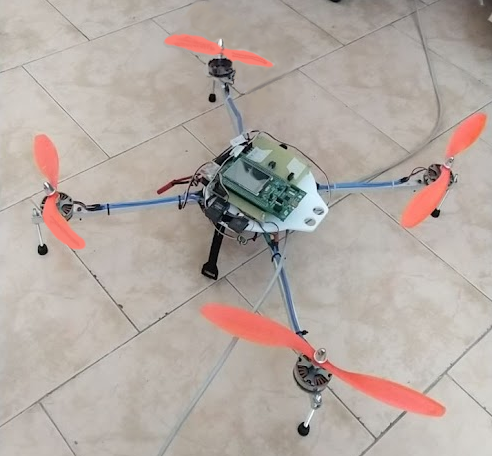
\includegraphics[width=0.5\textwidth]{drone_construction}
    \caption{Конструкция на Платформата с 4 ротора}
    \label{fig:drone_construction}
\end{figure}



\FloatBarrier
\subsection{Платформа за управление на ъгъл на завъртане}
\FloatBarrier

Платформата за управление на ъгъл на завъртане има за цел да ни позволи лесно и безаварийно да изпробваме алгоритмите за управление на ъгъл на завъртане.

Платфомрата \autoref{fig:balance_construction} е изградена от дърво.
Състои се от Т образна основа с ограничители и въртяща част.
Основата е висока \(30cm\) и е съставена от 2 правоъгълни дървени профил(\(30x10x2.5cm\)) съединенин с винтове. 
Ограничителите ограничават максималният ъгъл, който въртящата част може да сключва с хоризонта в диапазона (\(\pm 40^{\circ}\)).
Оста на въртене представлява M8 болт.
Оста образува болтово съединение с основата, както и с лагерите на въртяащата част.
Въртящата част е съставена от правоъгълен дървен профил (\(60x2.5x3cm\)), с вложени 2 лагера 
(сачмен с дълбок канал \(8x22mm\), максимално статично натоварване \(138kg\) \cite{datasheet_bearing}),
като са пробити отвори за болтово съединяване на основите за безчетковите постояннотокови мотори,
както и отвори за болтово съединяване на основата на жироскопа и акселерометъра.
Останалите нужни компонении, като \textit{ESC (Electronic Speed Controller)} за моторите са прикрепени към рамената на въртящата
част използвайки кабелни превръзки (т.нар свински опашки), като е взето предвид балансиране на платформата,
чрез разпределение на тежеста на допълнителните елементи.

\begin{figure}[htpb!]
    \centering
    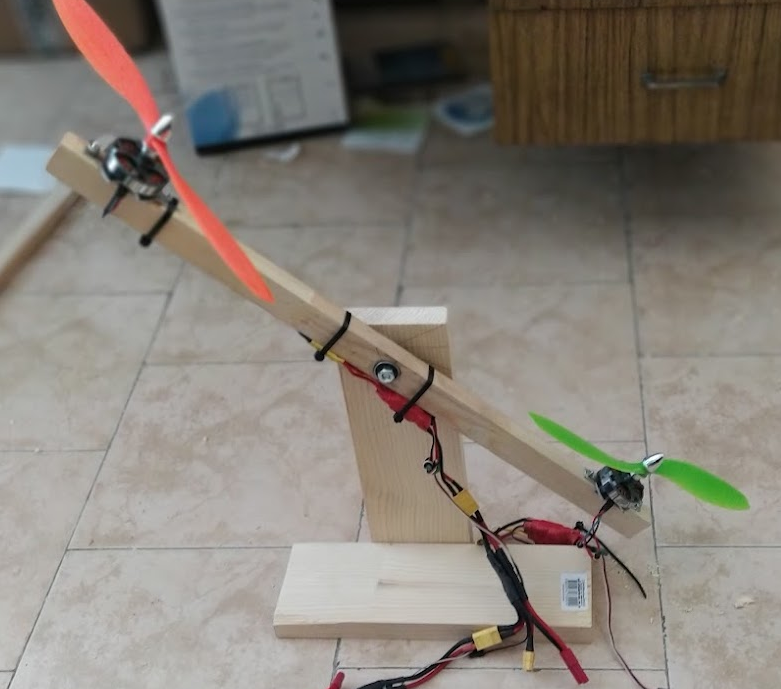
\includegraphics[width=0.7\textwidth]{balance_construction}
    \caption{Конструкция на платформата за управление на ъгъл}
    \label{fig:balance_construction}
\end{figure}

\FloatBarrier

